% Created 2018-04-20 Fri 23:10
% Intended LaTeX compiler: pdflatex
\documentclass[11pt, reqno]{amsart}
              

\usepackage[utf8]{inputenc}
\usepackage[T1]{fontenc}
\usepackage{graphicx}
\usepackage{grffile}
\usepackage{longtable}
\usepackage{wrapfig}
\usepackage{rotating}
\usepackage[normalem]{ulem}
\usepackage{amsmath}
\usepackage{textcomp}
\usepackage{amssymb}
\usepackage{capt-of}
\usepackage{hyperref}
\usepackage[newfloat]{minted}
\usepackage{caption}
\author{Yi Zhang}
\date{\today}
\title{\textbf{Stan} demo: Walk-on-sphere solution of Laplace equation}
\hypersetup{
 pdfauthor={Yi Zhang},
 pdftitle={\textbf{Stan} demo: Walk-on-sphere solution of Laplace equation},
 pdfkeywords={},
 pdfsubject={},
 pdfcreator={Emacs 25.3.1 (Org mode 9.1.3)}, 
 pdflang={English}}
\begin{document}

\maketitle
\tableofcontents


\section{Background}
\label{sec:org46c340c}
This \texttt{Stan} demo is a translation of one of my previosu R
projects, implementing the Walk-on-sphere(WOS) method to solve
the Laplace equation on a rectangle. This is the so-called
probabilistic mesh-free method for PDE solution. Essentially
the probabilistic interpretations of Laplace equation says
the solution is the mean of exit-points' function values of
Brownian motion. Instead of sampling the path of the
Brownian motion, we only need to sample the exit-points of
the Brownian motion that beginning at the location where we
wish to find PDE solution. This is a simplified version of
\textbf{Feyman-Kac formula}, which connects parabolic PDE with
Brownian motion. Since there is no inference, we run
\texttt{Stan} with \texttt{num\_samples=1} and \texttt{algorithm=fixed\_param}.


Specifically, we solve 

\begin{align*}
        \nabla^2 u(x ,y) = 0, & \quad \forall (x, y)\in \Omega= [0, 1] \times [0, 1],\\
        u = 0        ,& \quad \forall x=0,\\
        u = 0        ,& \quad \forall x=1,\\
        u = 0        ,& \quad \forall y=0,\\
        u = 75x      ,& \quad \forall y=1, x\in [0, 2/3],\\
        u = 150(1-x) ,& \quad \forall y=1, x\in [2/3, 1],
\end{align*}

\section{Model source code}
\label{sec:orga54cca9}
\begin{minted}[breaklines=true,fontsize=\footnotesize,breakanywhere=true]{stan}
/* This Stan demo of probalistic appraoch of PDE solution.
   It uses Walk-on-sphere method to calculate Laplace equ
   solution on a rectangle.
 */

/* run with */
/* .harmonic sample num_samples=1 algorithm=fixed_param data file=./harmonic.data.R */
functions {
  real[] rect_boundary_x() {
    real xb[2] = { 0.0, 1.0 };  /* rectangle boundary */
    return xb;
  }
  real[] rect_boundary_y() {
    real yb[2] = { 0.0, 1.0 };  /* rectangle boundary */
    return yb;
  }
  real bc(real x, real y) {
    real xb[2] = rect_boundary_x();
    real yb[2] = rect_boundary_y();
    real val;
    if (x == xb[1]) {           /* left boundary */
      val = 0.0;
    } else if ( x == xb[2]) {   /* right boundary */
      val = 0.0;
    } else if ( y == yb[1]) {   /* lower boundary */
      val = 0.0;
    } else if ( y == yb[2]) {   /* upper boundary */
      if (x <= 2.0/3.0)
        val = 75*x;
      else
        val = 150 * (1-x);
    }
    return val;
  }

  real rectangle_wos_rng(real x, real y, real tol) {
    real xb[2] = rect_boundary_x();
    real yb[2] = rect_boundary_y();
    real res[3] = {x, y, 0.0};
    real dist[4] = { xb[2] - res[1], res[1] - xb[1], yb[2] - res[2], res[2] - yb[1]};
    real r = min(dist);
    real val;
    while (r > tol) {
      real theta = uniform_rng(0, 2*pi());
      res[1] = res[1] + r * cos(theta);
      res[2] = res[2] + r * sin(theta);
      dist = { xb[2] - res[1], res[1] - xb[1], yb[2] - res[2], res[2] - yb[1]};      
      r = min(dist);      
      res[3] = r;
    }
    if (dist[1] < tol ) {       /* right boundary */
      res[1] = xb[2];
    } else if (dist[2] < tol ) { /* left boundary */ 
      res[1] = xb[1];
    } else if (dist[3] < tol ) { /* upper boundary */ 
      res[2] = yb[2];
    } else if (dist[4] < tol ) { /* lower boundary */
      res[2] = yb[1];
    }
    val = bc(res[1], res[2]);
    res[3] = val;
    return val;
  }
}

data{
  real tolerance;
  int m;
  int n;
  int N;
}

transformed data {
  vector[N] bcsample;
  real x;
  real y;
  real hm = 1.0/m;
  real hn = 1.0/n;
  real sol;
  for ( i in 1:m+1 ) {
    for ( j in 1:n+1 ) {
      x = (i-1)*hm;
      y = (j-1)*hn;
      for ( k in 1:N ) {
        bcsample[k] = rectangle_wos_rng(x, y, tolerance);        
      }
      sol = mean(bcsample);
    }
  }
}
\end{minted}

\section{Results}
\label{sec:org1198baa}
With the data file input
\begin{minted}[breaklines=true,fontsize=\footnotesize,breakanywhere=true]{r}
tolerance <- 0.00001                    # close-to-boundary tolerance
m <- 20                                 # nb. of grids in x-dir
n <- 20                                 # nb. of grids in y-dir
N <- 5000                               # samples to take
                                        # for each solution
\end{minted}
the following plot shows the solution surface.
\begin{center}
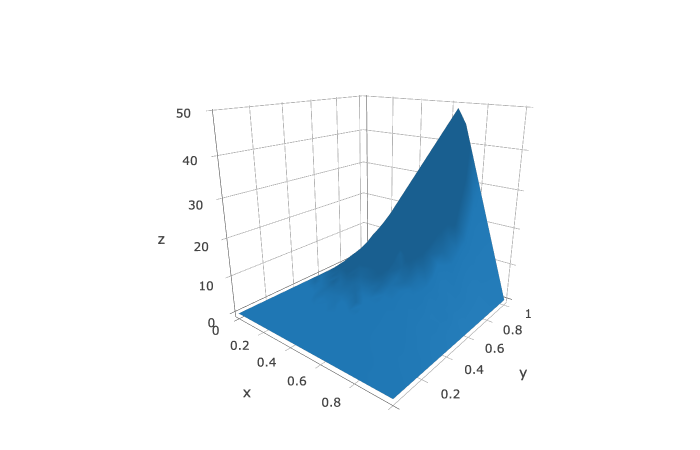
\includegraphics[width=.9\linewidth]{harmonic.png}
\end{center}
\end{document}
